\documentclass[11pt]{article}
\usepackage{amssymb, amsmath, libertine, hyperref, xcolor, booktabs, enumitem, microtype}
\usepackage[T1]{fontenc}
\usepackage[margin=1in]{geometry}
\usepackage{tikz}
\newcommand{\gridxy}[4]{% xmin xmax ymin ymax -- gridlines exactly on the ticks
  \foreach \gX in {#1,...,#2} \draw[gray!25] (\gX,#3) -- (\gX,#4);
  \foreach \gY in {#3,...,#4} \draw[gray!25] (#1,\gY) -- (#2,\gY);}
\definecolor{dark-red}{rgb}{0.4,0.15,0.15}
\hypersetup{colorlinks, linkcolor=dark-red, citecolor=dark-red, urlcolor=dark-red}
\setlist[enumerate,1]{label=\textbf{\arabic*.}, leftmargin=*, itemsep=10pt}
\setlist[enumerate,2]{label=(\alph*), leftmargin=*, itemsep=4pt, topsep=4pt}
\setlist[enumerate,3]{label=(\roman*), leftmargin=*, itemsep=2pt, topsep=2pt}
\pagestyle{empty}

\newcommand{\prob}[1]{\medskip\noindent\textbf{\large #1}\par\smallskip}

\begin{document}

\begin{center}
{\Large\bfseries Math 111: Calculus \quad Homework 3}\\[4pt]
{Due Friday, October 30 by 10:00\textsc{p.m.} via Gradescope}
\end{center}

\medskip
\noindent\textbf{Covers} Active Calculus \S3.3, \S3.4, and \S3.6. Problems~1 and~4 use
only \S3.3, which we cover on Monday, October~12, so you can do them before the break.
Problem~2 uses \S3.4 (Monday, October~26). Problem~3 can be done with the tools of \S3.3
if you follow the steps given; \S3.6 (Wednesday, October~28) will make it feel routine.
\textbf{No work is expected over fall break.}

\smallskip
\noindent\textbf{Before you start.} Write in sentences and paragraphs, as an
explanation another student in this course could read and follow. Draw diagrams large
and label them. You are encouraged to work with classmates; cite everyone you worked
with, and write your solutions independently --- duplicated solutions are an Honor
Principle violation. Each problem is marked holistically on the 0--5 scale, with up
to two further points for the quality of the writing. If you need an extension, use
the \href{https://docs.google.com/forms/d/e/1FAIpQLSfIfgx44SFtUzefTNr-80yz35MVJaUqQttt96xVTU5mCQCOgg/viewform}{extension
form} \emph{before} the deadline.

\bigskip\hrule\bigskip

%%%%%%%%%%%%%%%%%%%%%%%%%%%%%%%%%%%%%%%%%%%%%%%%%%%%%%%%%%%%%%%%%%%%%%%%%%%%%%%%
\prob{1. Everything about $f$ from a picture of $f'$}

Below is the graph of the \emph{derivative} $f'$ of a function $f$ on $[0,8]$. This is
not a graph of $f$. No formula is given for either.

\smallskip
\begin{center}
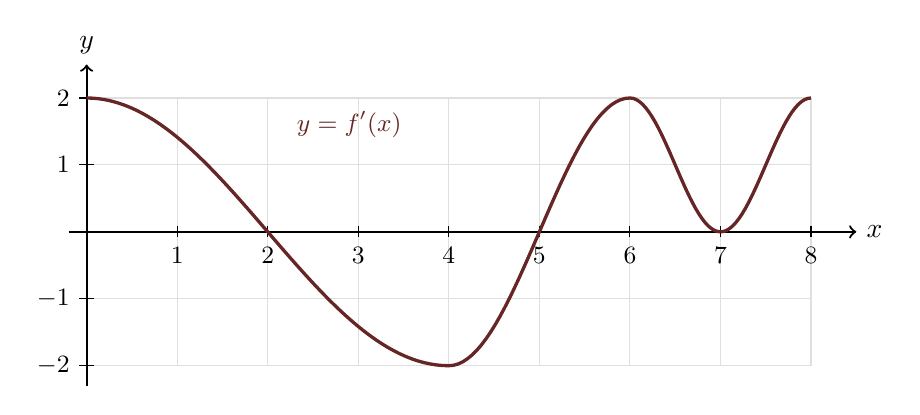
\begin{tikzpicture}[x=1.15cm,y=0.85cm]
  \gridxy{0}{8}{-2}{2}
  \draw[->,thick] (-0.2,0) -- (8.5,0) node[right] {$x$};
  \draw[->,thick] (0,-2.3) -- (0,2.5) node[above] {$y$};
  \foreach \x in {1,...,8} \draw (\x,0.08) -- (\x,-0.08) node[below,font=\small] {\x};
  \foreach \y in {-2,-1,1,2} \draw (0.08,\y) -- (-0.08,\y) node[left,font=\small] {$\y$};
  \draw[very thick, dark-red, domain=0:4, samples=60] plot (\x,{2*cos(deg(pi*\x/4))});
  \draw[very thick, dark-red, domain=4:6, samples=40] plot (\x,{-2*cos(deg(pi*(\x-4)/2))});
  \draw[very thick, dark-red, domain=6:7, samples=30] plot (\x,{1+cos(deg(pi*(\x-6)))});
  \draw[very thick, dark-red, domain=7:8, samples=30] plot (\x,{1-cos(deg(pi*(\x-7)))});
  \node[dark-red,font=\small] at (2.9,1.6) {$y=f'(x)$};
\end{tikzpicture}
\end{center}

\begin{enumerate}[resume]
\item[]
\begin{enumerate}
\item Find every critical number of $f$ in $(0,8)$. Classify each as a local maximum, a
local minimum, or neither, and justify each classification from the graph of $f'$.

\item On which intervals is $f$ concave up, and on which is it concave down? Where does
$f$ have inflection points? Explain how you read each answer off the graph of $f'$.

\item One of the critical numbers you found in (a) is also an inflection point. Describe
in words what the graph of $f$ looks like near that point, and name a simple formula
whose graph behaves the same way near $0$.

\item Where on $[0,8]$ does $f$ take its \emph{largest} value? Your work in (a) should
narrow it down to two candidates but not decide between them. Say what the two
candidates are, say exactly what further information about $f$ would decide it, and then
make your best guess from the picture of $f'$, explaining what in the picture you are
using. (We will have a precise tool for this in November.)

\item Suppose $f(0)=1$. Sketch a graph of $f$ on $[0,8]$ that is consistent with
everything above. Mark the critical points and inflection points.
\end{enumerate}
\end{enumerate}

%%%%%%%%%%%%%%%%%%%%%%%%%%%%%%%%%%%%%%%%%%%%%%%%%%%%%%%%%%%%%%%%%%%%%%%%%%%%%%%%
\newpage
\prob{2. A family of functions}

For each constant $a$, let
\[
g_a(x) = x + \frac{a}{x}, \qquad x > 0 .
\]
Keep $a$ as a letter throughout; do not pick a value unless a part asks you to.

\begin{enumerate}[resume]
\item[]
\begin{enumerate}
\item Suppose $a>0$. Find the critical number(s) of $g_a$ on $(0,\infty)$ in terms of $a$,
and classify each. Then compute $g_a''$ and say what it tells you about the shape of the
graph.

\item Still with $a>0$: as $a$ varies, the lowest point on the graph of $g_a$ moves.
Show that all of these lowest points lie on a single line, and find its equation. On one
set of axes, sketch $g_1$, $g_4$, and $g_9$ together with that line.

\item Now suppose $a<0$. Does $g_a$ have any critical numbers on $(0,\infty)$? Describe
the shape of the graph of $g_a$ in words (increasing or decreasing? concave up or down?),
justifying each claim from $g_a'$ and $g_a''$. What happens when $a=0$?

\item Find the value of $a$ for which the lowest point of $g_a$ occurs at $x=3$, and say
what that lowest value is.
\end{enumerate}
\end{enumerate}

%%%%%%%%%%%%%%%%%%%%%%%%%%%%%%%%%%%%%%%%%%%%%%%%%%%%%%%%%%%%%%%%%%%%%%%%%%%%%%%%
\prob{3. Why aren't cans shaped like that?}

A cylindrical can with radius $r$ and height $h$ holds volume $V=\pi r^2h$. Its metal
consists of a top and a bottom (each a disk of area $\pi r^2$) and a side (area $2\pi
rh$). Throughout, the volume $V$ is a fixed positive constant.

\begin{enumerate}[resume]
\item[]
\begin{enumerate}
\item Use $V=\pi r^2h$ to write the total surface area $S$ as a function of $r$ alone.
Find the value of $r$ that makes $S$ as small as possible, explain how you know it is a
minimum and not a maximum, and show that at this radius the height equals the diameter.

\item In 1987 a mathematics professor wrote to the Carnation company asking why their
cans are not shaped that way. The company's reply is reproduced in Peter Keep's
\emph{Discover Calculus}:
\href{https://www.discovercalculus.com/web/app-CarnationLetter.html}{discovercalculus.com/web/app-CarnationLetter.html}.
Read it. The letter's second reason is that the top and bottom must be made of thicker
metal than the side. Model that: suppose the metal for the top and bottom costs $k$
times as much per square unit as the metal for the side, where $k>1$, so the cost of a
can is proportional to
\[
C = k\cdot 2\pi r^2 + 2\pi r h .
\]
Find the radius that minimizes $C$, and show that at that radius the ratio of height to
diameter is exactly $k$. Does this push the best can toward being taller or shorter than
the answer in (a)? Is that the direction the letter says?

\item Choose \emph{two} of the letter's other reasons. For each, say in a sentence or two
which way it pushes the shape of the can (taller and thinner, or shorter and wider, or
neither), and whether you think it could be built into a function to minimize the way
reason two was in (b). If yes, say roughly what you would add to $C$; if no, say what makes
it hard to put into a formula.

\item The optimization in (a) is correct mathematics, and the cans on a grocery shelf are
not shaped like its answer. In a short paragraph, say what that does and does not tell
you about the usefulness of optimization.
\end{enumerate}
\end{enumerate}

%%%%%%%%%%%%%%%%%%%%%%%%%%%%%%%%%%%%%%%%%%%%%%%%%%%%%%%%%%%%%%%%%%%%%%%%%%%%%%%%
\newpage
\prob{4. Examples to order, and a broken argument}

\begin{enumerate}[resume]
\item[]
\begin{enumerate}
\item Give a function $f$ that has a critical number at $x=0$ because $f'(0)$ is
\emph{undefined} (not because it is $0$), and that has neither a local maximum nor a local
minimum at $0$. Explain how you know both things.

\item Give a function that is differentiable on the open interval $(0,1)$ and has neither a
global maximum nor a global minimum on $(0,1)$. Explain why, and then explain why the same
function \emph{does} have both on the closed interval $[0,1]$.

\item A student submits the following.

\smallskip
\begin{quote}
\textbf{Claim.} If $f''(c)=0$, then $f$ has an inflection point at $x=c$.

\textbf{Argument.} Since $f''(c)=0$, the second derivative is neither positive nor
negative at $c$. So at $c$ the graph of $f$ is neither concave up nor concave down. So the
concavity of $f$ changes at $c$, which is what an inflection point is.
\end{quote}
\smallskip

Identify the \emph{first} sentence of the argument that is wrong, and say precisely what
is wrong with it. Then give a specific function showing the claim is false, and check
your example. Finally, state a correct claim of the same shape --- a condition on $f''$
that \emph{does} guarantee an inflection point at $c$ --- and say why it is true.
\end{enumerate}
\end{enumerate}

\end{document}
